\chapter{Evaluation}
\label{chp:evaluation}
% Be warned that many projects fall down through poor evaluation. Simply building a system and documenting its design and functionality is not enough to gain top marks. It is extremely important that you evaluate what you have done both in absolute terms and in comparison with existing techniques, software, hardware etc. This might involve quantitative evaluation, for example based on numerical results, performance etc. or something more qualitative such as expressibility, functionality, ease-of-use etc. At some point you should also evaluate the strengths and weaknesses of what you have done. Avoid statements like "The project has been a complete success and we have solved all the problems asssociated with blah...; - you will be shot down immediately! It is important to understand that there is no such thing as a perfect project. Even the very best pieces of work have their limitations and you are expected to provide a proper critical appraisal of what you have done.

\section{Strengths and weaknesses}

The GCV signature has been successfully used on some of the networks and it helped us get valuable insights. The best results have been obtained on the WTN networks, followed by the PPI and metabolic networks. Overall, the main achievements of this project are as follows:
\begin{itemize}
 \item The development of the mathematical model of the GCV signature followed by the implementation and parallelisation of the algorithm that computes it.
 \item The use of a rigorous methodology for the analysis of GCV correlations that helped us uncover insights from the network data.
 \item The results and interpretations presented for the economic, protein interaction and metabolic networks.
 \item The quantitative evaluation of the GCV signature (sections \ref{sec:eval_clust} and \ref{sec:eval_classify}).
\end{itemize}

However, the GCV signature has inherent limitations and weaknesses. The main deficiencies with our methodology are:
\begin{itemize}
 \item A more effective normalisation method of the GCV can be designed. Such a normalisation method can take into account the size of the neighbourhood subgraph.
 \item A redundancy analysis of each GCV frequency has not been made. This could tell us whether elements in the GCV vector are redundant and eliminating these will improve the GCV performance and remove noise.
 \item The GCV signature is only able to quantify the structure between the immediate neighbours of a node. It cannot capture the structure between nodes that are further away from the source node, at distances of 2 or more. 
 \item The implementation of the GCV computation is not parallelisable on a cluster of computers. The program is only able to spawn processes that run on multiple cores. Moreover, when using multiple processes for parallel GCV computation, most of the processes finish their share early while a few processes get stuck with computing GCVs for hub nodes. This problem could be overcome by redistributing the workload to the processes that finish early.
 \item The GCV signature is not able to capture any information in some of the networks, such as the enzyme-based metabolic network. Further research needs to be done in order to understand why that is the case.
 \item The results we got for the WTN, PPI and Metabolic networks need more supporting experiments in order to validate the interpretations. 
\end{itemize}


\section{Evaluation of network clustering}
\label{sec:eval_clust}

Although the focus of this project is on using the GCV signature for uncovering hidden structures in the data analysed, we are also interested to find out whether the GCV can be used for clustering networks of different types. In this section, we evaluate the performance of the GCV signature on clustering the following types of random graphs:
\begin{itemize}
 \item Erd\H{o}s-R\'{e}nyi graphs (ER)
 \item Erd\H{o}s-R\'{e}nyi graphs with preserved degree distribution (ER-DD)
 \item Geometric graphs (GEO)
 \item Scale-free Barab\'{a}si-Albert graphs (preferential attachment) (SF-BA)
 \item Stickiness index-based graphs (STICKY)
\end{itemize}

For each model, we generate 30 different networks that are modelled from the 2010 World Trade network. These random networks have also been used in section \ref{sec:initial_experiments_rnd_nets} for computing the average network GCVs. For each one of the 150 generated networks, we compute 6 different signatures:
\begin{enumerate}
 \item Graphlet Cluster Vector (GCV)
 \item Degree Distribution
 \item Average clustering coefficient
 \item Spectral distribution
 \item Graphlet Frequency Vector (GFV).
 \item Graphlet Distribution Vector (GDV).  
\end{enumerate}

Calculating each of the 6 signatures requires a considerable amount of computation. This is the reason why we have chosen to generate the random networks from the WTNs, because these networks are small in comparison to the metabolic or PPI networks. Other networks such as the PPI networks are much larger and computation of all the signatures on 150 of these networks is very intense. 

After all signatures for the 150 networks have been calculated, the distance between each pair of networks is computed. All these entries are placed in a 150x150 distance matrix and 6 distance matrices are finally obtained, one for each signature. The distance matrices can be used for visualising the distances using \emph{Multi-dimensional scaling} or for performing Precision-Recall curve analysis or Receiver-Operating Characteristic (ROC) curve analysis. These results are presented in the next sections. 

The Relative Graphlet Frequency distance (RGFD) defined in section \ref{sec:rgfd} has been used as the distance metric between two Graphlet Frequency Vectors. For the distance metric between two Graphlet Distribution Vectors, we have used the Graphlet Correlation Distance defined in section \ref{pearsons_background}. This will be denoted as GCD73, because it uses information from all 73 orbits and in order to distinguish it from a similar metric called GCD-11 that has been developed by Yavero\u{g}lu et al \cite{yaverouglu2014revealing}. For the degree and spectral distributions, we have used as the Euclidean distance between the first 60 elements.\footnote{These distributions are in theory infinite so we decided to cap them at 60, since very little information is retained after this threshold.}

\section{Multi-dimensional scaling results}

Multi-dimensional scaling (MDS) refers to a series of visualisation techniques which attempts to represent $n$-dimensional data points into a 2D or 3D space such that the distances between them are preserved as much as possible. We computed 3D MDS plots for each of the 6 signatures using the \lstinline|Python Scikit| library which provides the function \lstinline|sklearn.manifold.MDS| that can perform the MDS transformation. 

Figures \ref{fig:gcv_mds} and \ref{fig:clust_coeff_mds} provide the 3D MDS plots for the GCV and the Clustering coefficient. For the GCV MDS plot, the ER networks are more spread compared to the other random graphs and clearly distanced from them. On the other hand, the distances between the ER-DD, STICKY and SF-BA graphs are really small, suggesting that the GCV signature cannot easily distinguish between these random networks. We also notice that the SF-BA random graphs have formed two different clusters. This phenomena might be explained by the fact that the SF-BA random graphs are very sensitive to the initial starting graph.  We therefore conclude that the GCV signature can only distinguish the ER networks from the rest. 

For the Clustering coefficient MDS, the data points are positioned in a nearly collinear fashion, because the clustering coefficient is a 1-dimensional signature. The ER-DD and Stickiness graphs show some degree of overlap\footnote{this fact is not completely obvious from the graph because the STICKY data points are covering the corresponding ER-DD data points.}, while the rest of the random graphs are clearly separated from each other. This means that the clustering coefficient is able to distinguish any two pairs of random graphs apart from a STICKY, ER-DD network pair.


\begin{figure}[H] 
  \captionsetup{width=8cm}
  \hspace{-2.0em}
  \begin{minipage}[b]{0.55\linewidth}
    \centering
    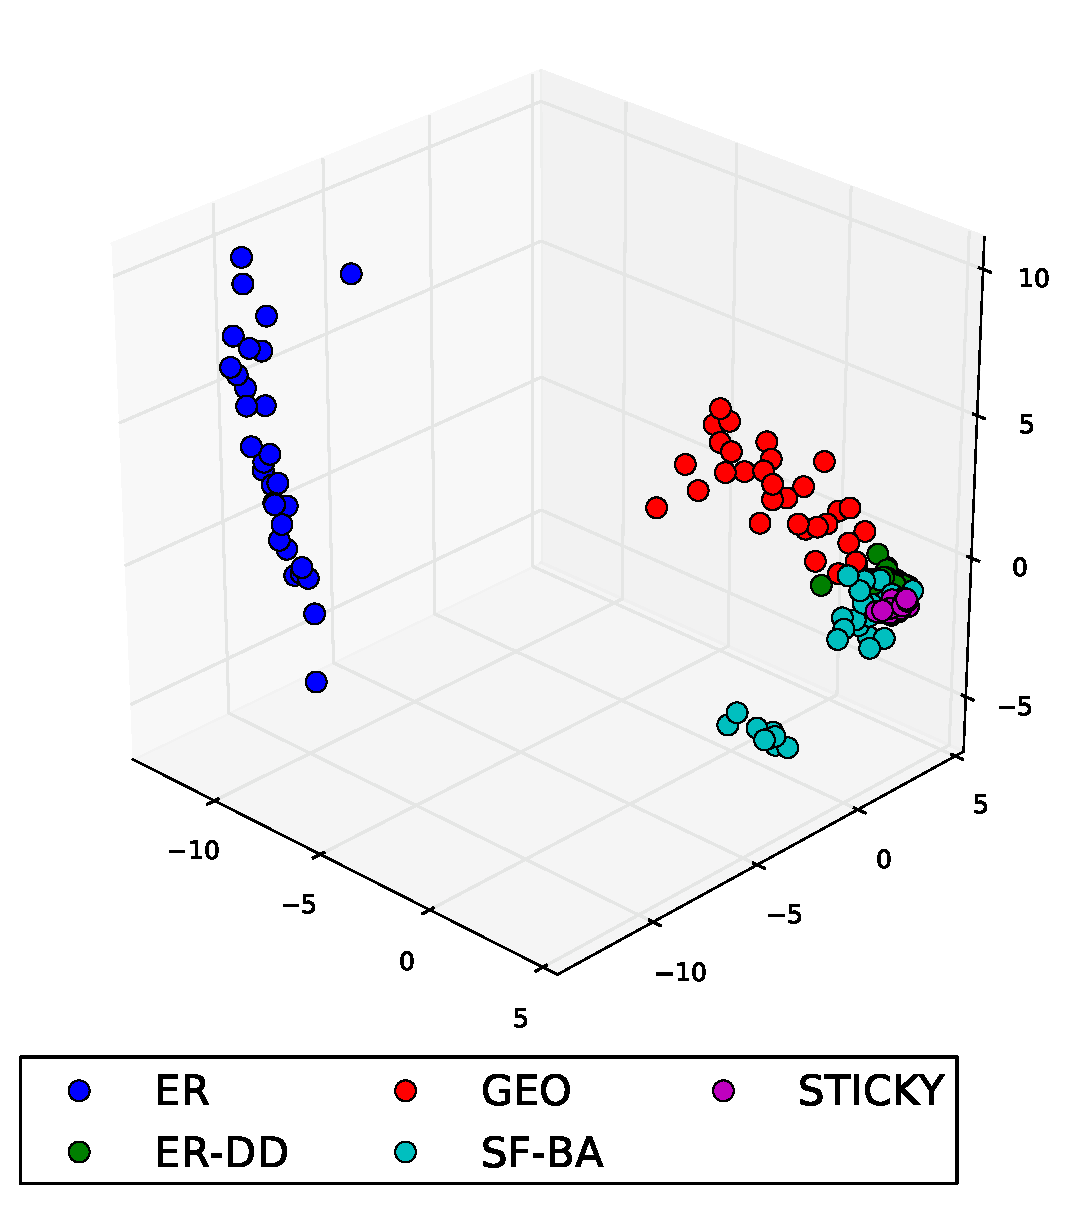
\includegraphics[scale=0.45]
    {../code/final_results/trade_2010_thresholded/eval_results/gcv_mds.pdf}
    \caption[Graphlet Cluster Vector MDS]{GCV MDS: The GCV signature cannot distinguish between ER-DD, GEO, SF and STICKY random graphs. The intra-cluster variance for ER networks is high.}
    \label{fig:gcv_mds}
%     \vspace{0.0ex}
  \end{minipage}%%
%   \hspace{0.5cm}
  \begin{minipage}[b]{0.55\linewidth}
    \centering
    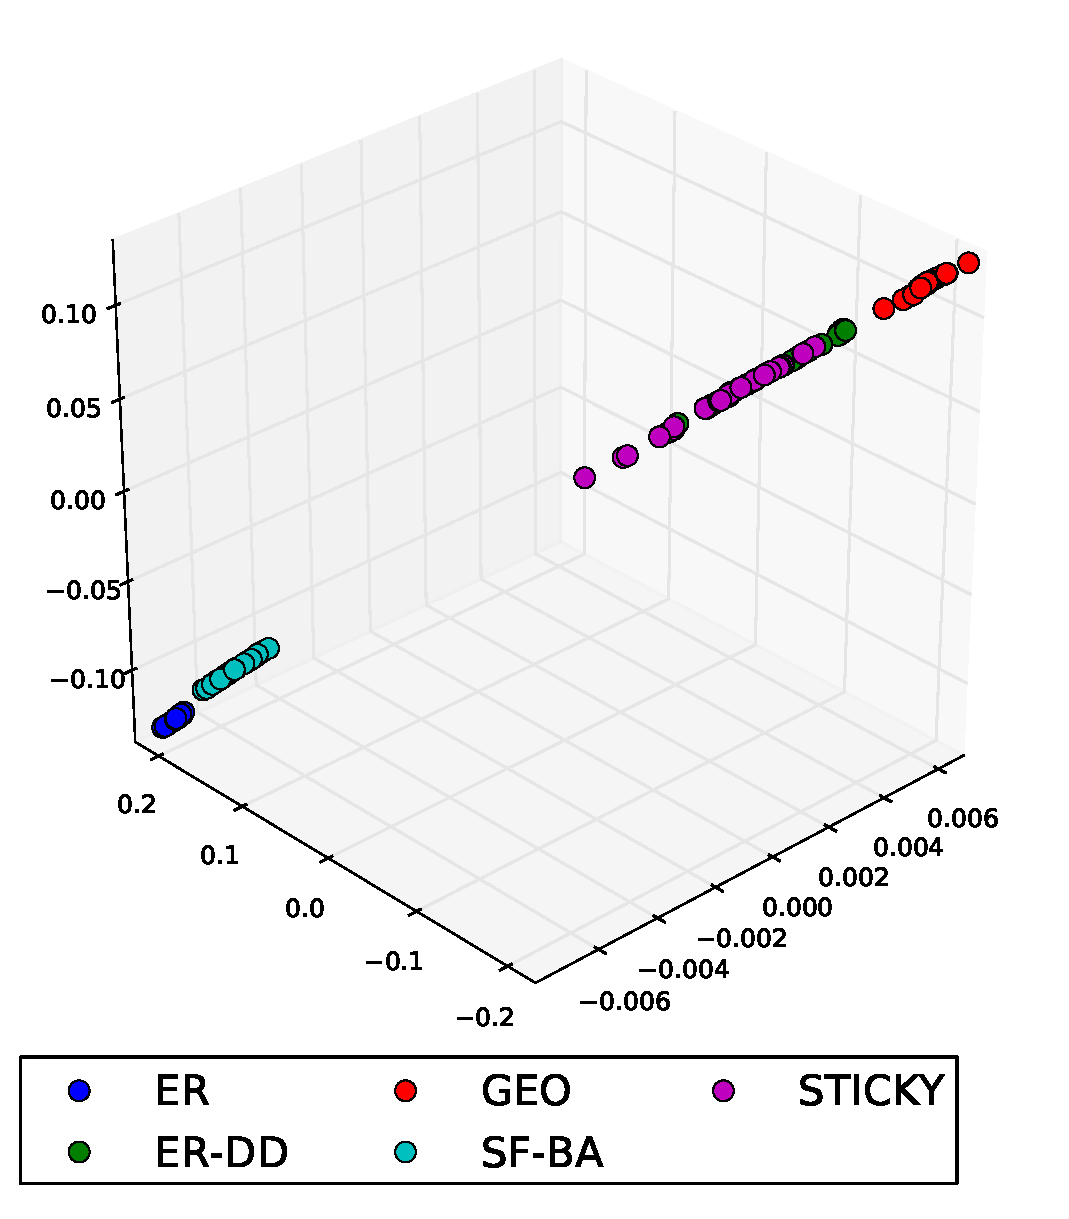
\includegraphics[scale=0.45]
    {../code/final_results/trade_2010_thresholded/eval_results/clust_coeff_mds.pdf}
    \caption[Clustering Coefficient MDS]{Clustering Coefficient MDS: The clustering coefficient cannot distinguish between ER-DD and STICKY random graphs (ER-DD points are hidden behind the STICKY points).}
    \label{fig:clust_coeff_mds}
%      \vspace{-1.0ex}
  \end{minipage} 
\label{fig:gcv_clust_mds} 
\end{figure}

The RGFD and GCD73 MDS plots are shown in figures \ref{fig:gfv_mds} and \ref{fig:gcd73_mds} respectively. The RGFD MDS shows that each of the clusters is clearly separated from the other, suggesting that RGFD is highly suitable for separating these types of networks. The GCD-73 metric is also suitable for clustering random networks, but the clusters display a higher variance.

\begin{figure}[H]
  \captionsetup{width=8cm}
  \hspace{-2.0em}
  \begin{minipage}[b]{0.55\linewidth}
    \centering
    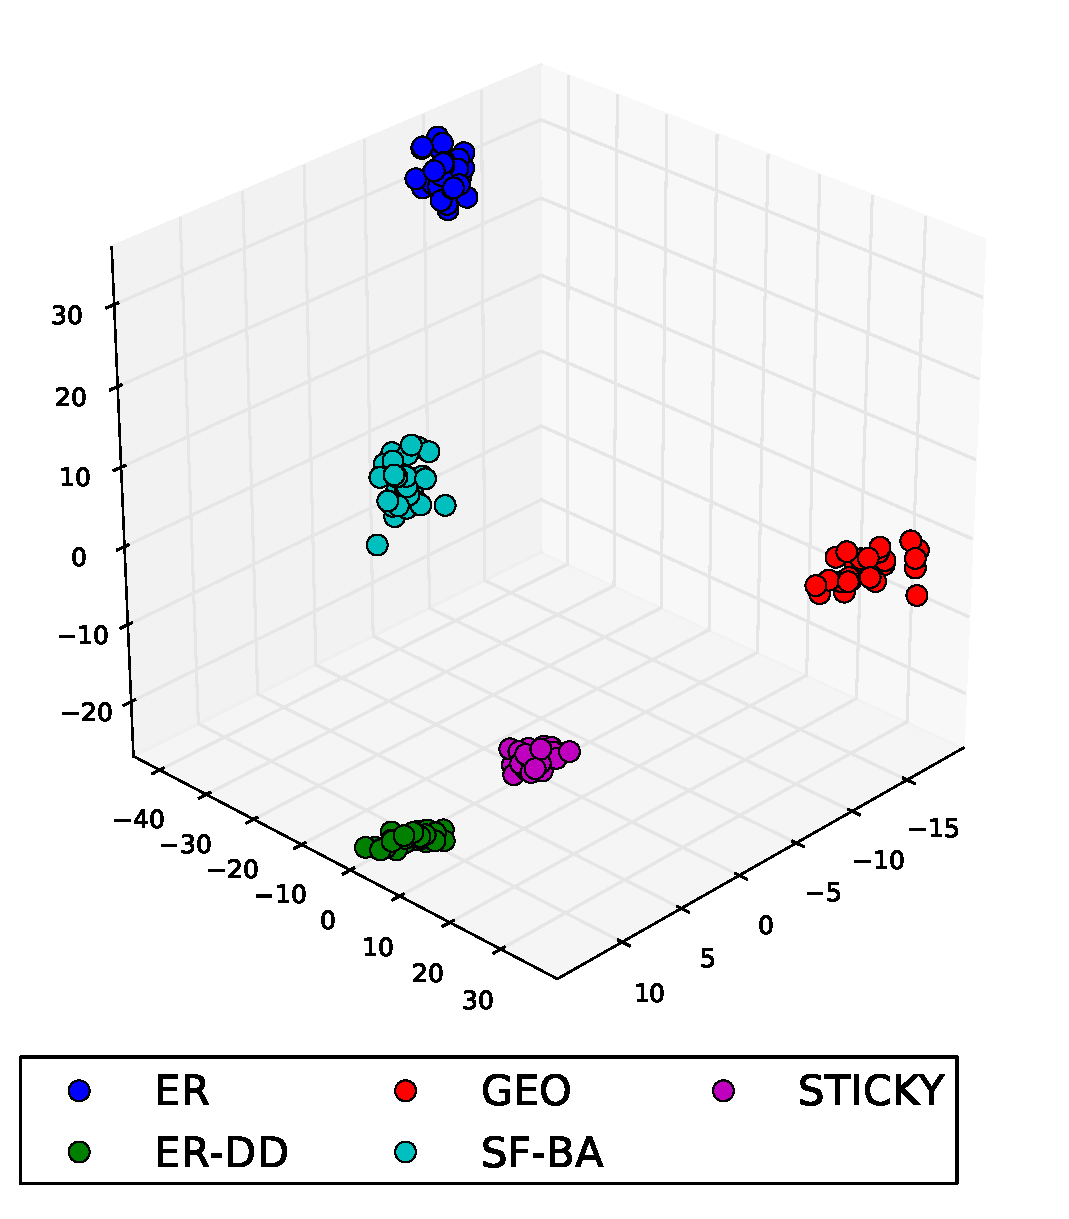
\includegraphics[scale=0.45]
    {../code/final_results/trade_2010_thresholded/eval_results/rgfd_mds.pdf}
    \caption[Relative Graphlet Frequency distance MDS]{RGFD MDS: The RGFD is clearly able to separate all the random network models. The intra-cluster variance is low.}
    \label{fig:gfv_mds}
  \end{minipage}%% 
%   \hspace{1.0em}
  \begin{minipage}[b]{0.55\linewidth}
    \centering
    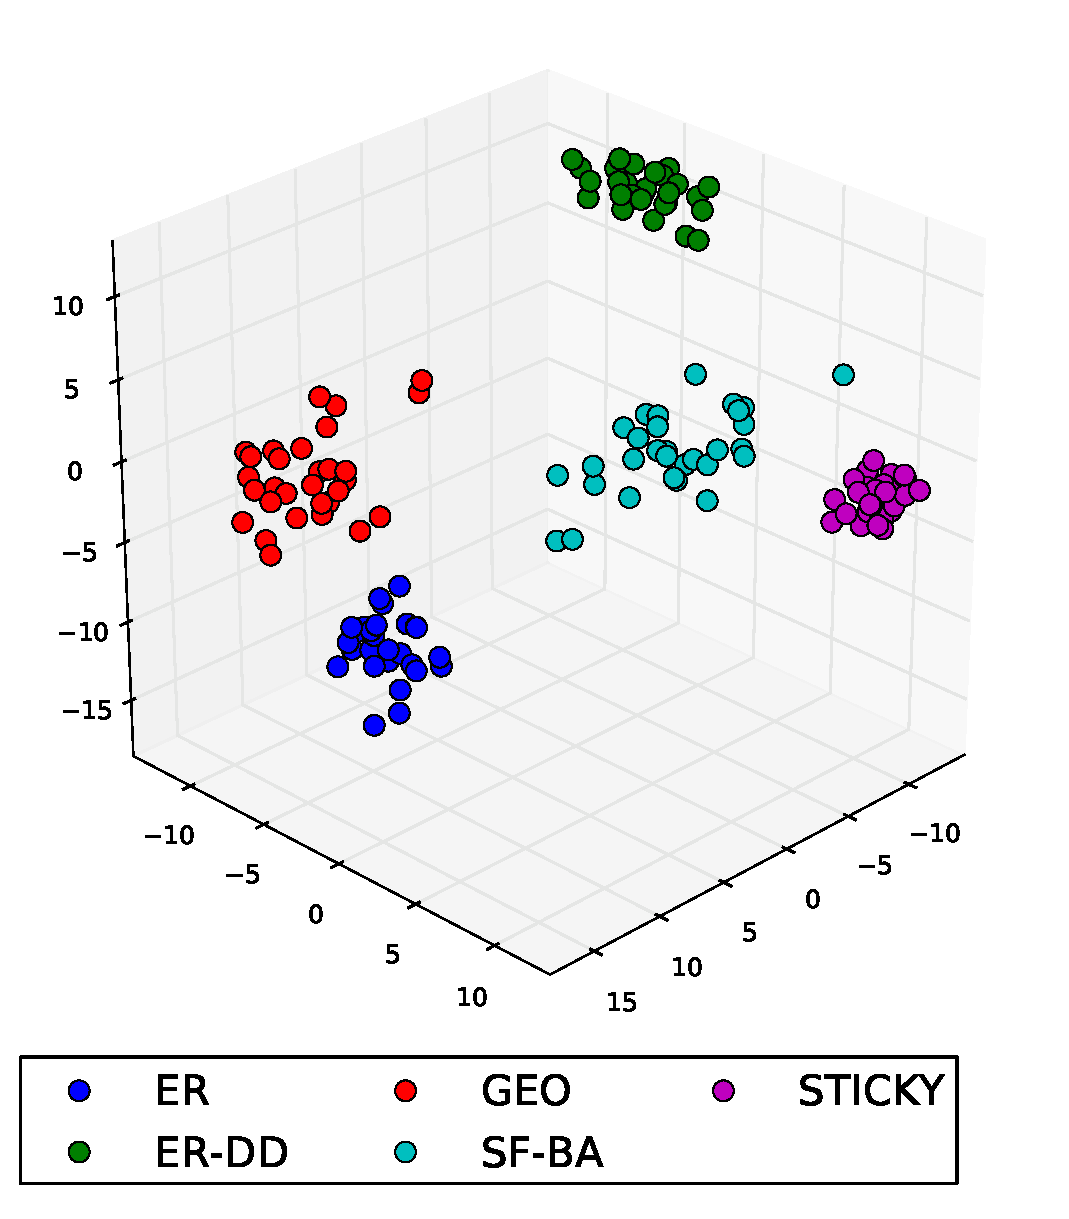
\includegraphics[scale=0.45]
    {../code/final_results/trade_2010_thresholded/eval_results/gcd73_mds.pdf}
    \caption[Graphlet correlation distance (GCD73) MDS]{GCD73 MDS: The GCD73 metric is also efficient at clustering random networks although the clusters are more spread around.}
    \label{fig:gcd73_mds}
%     \vspace{-1.0ex}
  \end{minipage} 
  \label{fig:rgfd_gdv_mds}
\end{figure}

Figures \ref{fig:degree_distrib_mds} and \ref{fig:spectral_distrib_mds} provide the 3D MDS plots for the Degree distribution and the Spectral Distribution signatures. The GEO and ER clusters in the Degree distribution MDS show a certain degree of overlap, although in reality there is much less overlap because the viewing angle is unsuitable\footnote{We tried to capture the image from other angles but that resulted in other clusters colliding.}. In the Spectral Distribution MDS, we notice that the ER and GEO clusters are very close to each other, suggesting that the Spectral Distribution cannot easily distinguish between these two types of random networks. However, the other clusters are clearly separated from each other.  

\begin{figure}[H]
  \captionsetup{width=8cm}
  \hspace{-2.0em}
  \begin{minipage}[b]{0.55\linewidth}
    \centering
    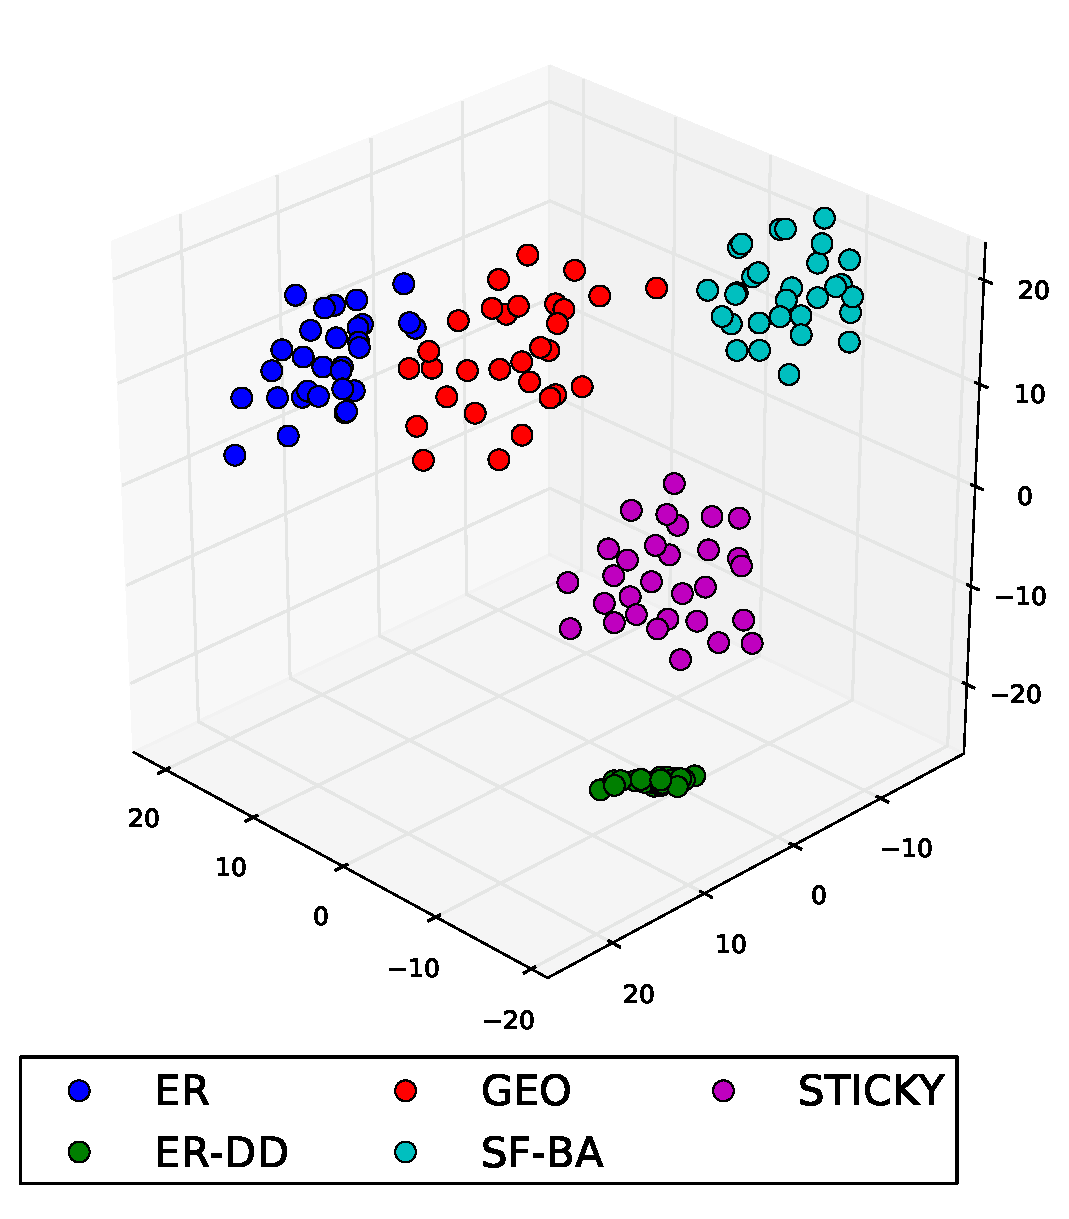
\includegraphics[scale=0.45]
    {../code/final_results/trade_2010_thresholded/eval_results/deg_distrib_mds.pdf}
    \caption[Degree Distribution MDS]{Degree Distribution MDS: Most of the clusters are clearly separated although the intra-cluster variance for ER, GEO, SF-BA and STICKY is high.}
    \label{fig:degree_distrib_mds}
  \end{minipage}%% 
  \begin{minipage}[b]{0.55\linewidth}
    \centering
    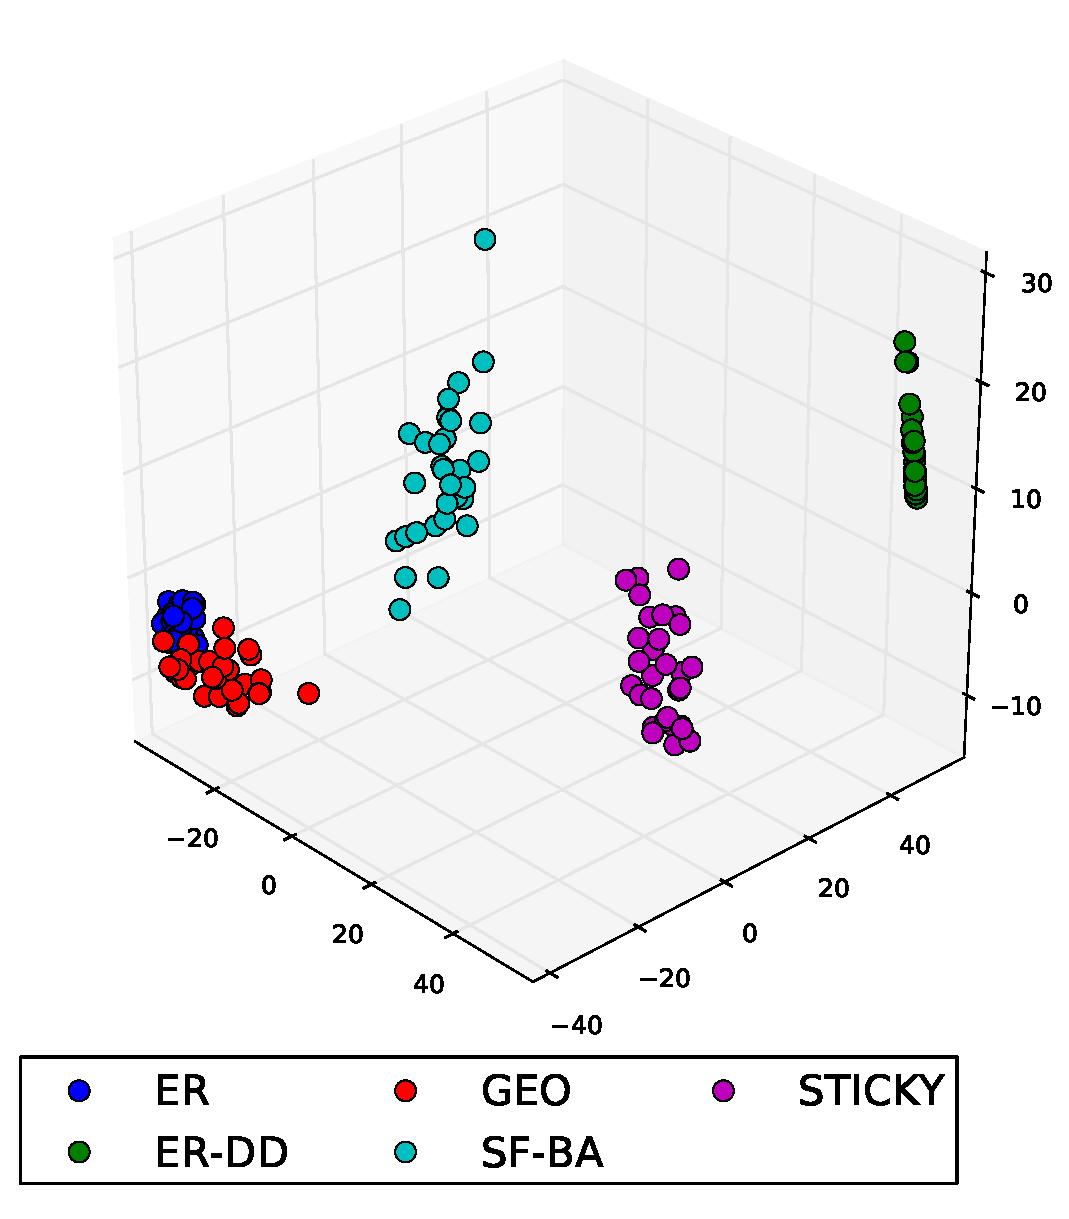
\includegraphics[scale=0.45]
    {../code/final_results/trade_2010_thresholded/eval_results/spectral_distrib_mds.pdf}
    \caption[Spectral Distribution MDS]{Spectral Distribution MDS: The spectral distribution cannot distinguish between ER and GEO random graphs. The other pairs of clusters are clearly separated.}
    \label{fig:spectral_distrib_mds}
%     \vspace{-1.0ex}
  \end{minipage} 
\end{figure}

\section{Precision-Recall curve}

MDS plots are only useful for visualising the distance matrices. However, one can test how well a distance measure groups networks of the same type by using the Precision-Recall curve. Starting from the 150x150 distance matrix, a Precision-Recall curve analysis can be performed in the following manner:
\begin{enumerate}
 \item one searches for the minimum and maximum distance in the distance matrix.
 \item for small increments of parameter $\epsilon$ such that $ min \le \epsilon \le max$, if the distance between two networks is smaller than $\epsilon$ then the pair of networks is retrieved
  \begin{enumerate}
  \item Precision is calculated as the fraction of the correctly retrieved pairs (i.e.\ grouping networks from the same model)
  \item Recall is calculated as the fraction of the correctly retrieved pairs over all the correct ones. 
  \end{enumerate}
 \item The Precision-Recall curve is plotted using the values calculated so far. 
 \item The Area under Precision-Recall (AUPR) can be calculated using the following formula:
	$$ AUPR = AUPR + 0.5 * (REC[k]-REC[k-1])*(PREC[k]+PREC[k-1]) $$
\end{enumerate}

We chose to perform a Precision-Recall curve analysis because it is known to be more robust to large numbers of negatives than Receiver Operator Characteristic (ROC) curve analysis \cite{davis2006relationship}. In our case negatives are pairs of networks that are grouped together although they belong to different random models.

Figure \ref{fig:prec_rec} shows the precision-recall curve for the six signatures calculated from their distance matrices. Our novel GCV signature has a generally low precision compared to the other signatures, as the precision decreases a lot in the recall range [0.2 -- 0.5]. This result was expected from our signature, since the MDS plots showed that it cannot easily distinguish between ER-DD, STICKY, SF-BA and GEO random graphs (figure \ref{fig:gcv_mds}). The best-performing signature is actually the RGFD, which has a precision of 1 for any recall value in range [0 -- 1]. Note that this is only faintly seen on the plot, because the GCD73 line overwrites it.
\begin{figure}[H]
  \hspace{-1.5em}
%   \centering
  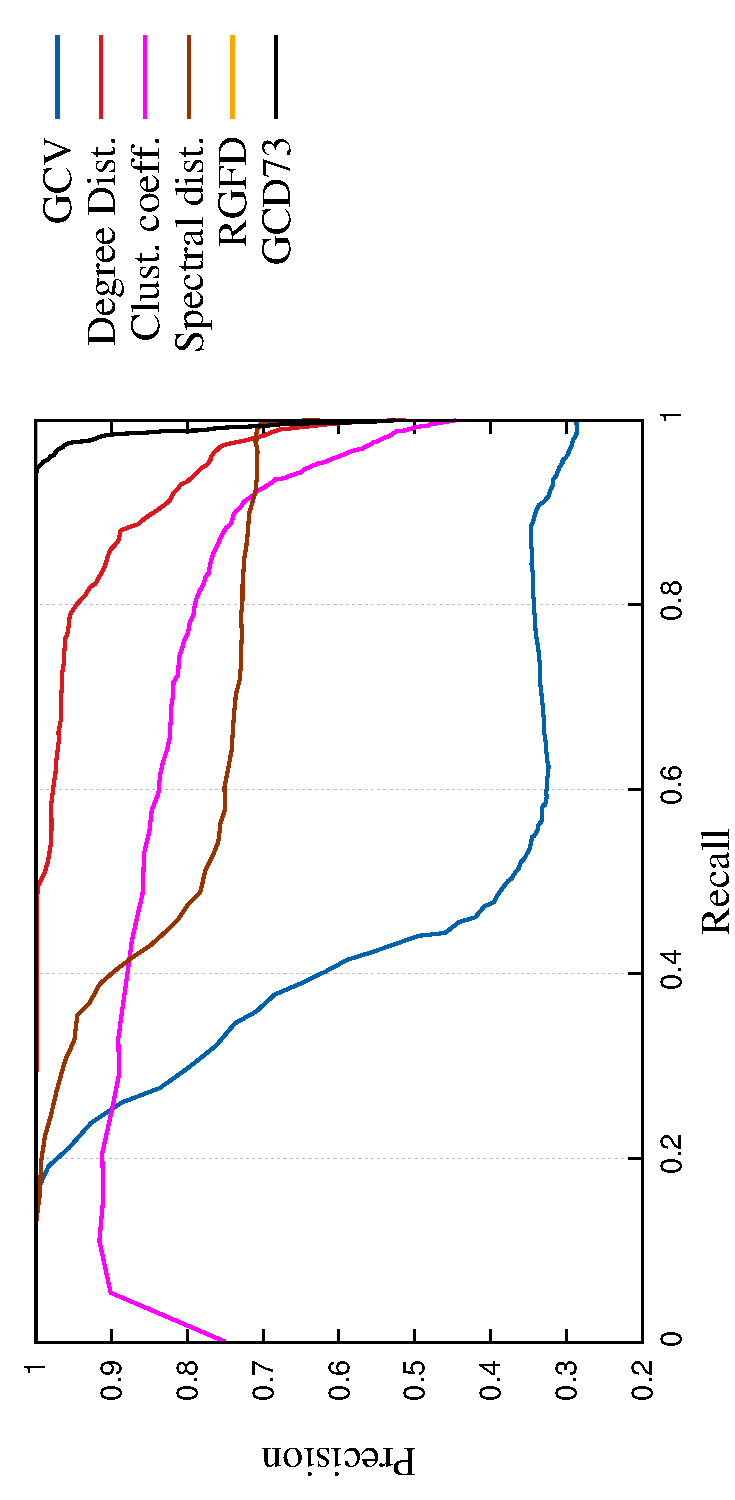
\includegraphics[scale=0.7, angle=-90]
  {../code/final_results/trade_2010_thresholded/eval_results/prec_rec_all_rnd_rew_02.pdf}
  \caption[Precision-Recall curves for GCV and 5 other signatures]{Precision-Recall curves for 6 different signatures: Graphlet Cluster Vector (GCV), Degree Distribution, Clustering Coefficient, Spectral Distribution, the Relative Graphlet Frequency distance (RGFD) and the Graphlet Correlation distance which uses the 73 automorphism orbits (GCD73). The best performing signature is the RGFD which has a value of 1 for any recall value. However, this is not clearly seen in the plot because the GCD73 line overwrites it. The GCV signature has the worst performance particularly in the range [0.25--1].}
  \label{fig:prec_rec}
\end{figure}

Table \ref{tab:aupr} shows the table of AUPR values for each of the signatures. The higher the AUPR, the better the signature is at distinguishing between different clusters. The best-performing distance measure is the RGFD that uses the \emph{Graphlet Frequency Vector} of the random network. It has a perfect AUPR of 1.0, which is expected because the RGFD MDS plot showed it can clearly distinguish all the random graphs generated. On the opposite end, our GCV signature has the worst AUPR of only 0.575. This suggests that the GCV signature is not suitable for clustering random networks generated from the WTN. 

\begin{table}[H]
  \centering
  \begin{tabular}{  c | c }
    GCV & 0.575\\
    \hline
    Degree Distribution & 0.949\\
    Clustering Coefficient & 0.829\\
    Spectral Distribution & 0.840\\
    RGFD & \textbf{1.0}\\
    GCD73 & 0.994\\
  \end{tabular}
  \caption{AUPR table for the GCV and other signatures. The best AUPR has been obtained using the GCD73 signature, which has an AUPR of 0.994. On the other hand, our GCV signature performed worst with an AUPR of 0.575.}
  \label{tab:aupr}
\end{table}


\section{Robustness testing}

This section evaluates the robustness of the six signatures. The same Precision-Recall curve analysis is performed, this time with data that is noisy, incomplete or when the signatures are approximated. However, because of the sheer number of experiments performed, only the final AUPR values are plotted. The methodology is similar to that performed by Yavero\u{g}lu et al. on the short GCD-11 signature \cite{yaverouglu2014revealing}. 

\subsection{Network Rewiring}

In most real-life scenarios the data we have to work with is noisy. In order to evaluate the GCV robustness to noise, we take each of our initial 150 generated random networks and rewire the edges with a probability $p$, for different values of $p$ between 0 and 1. When rewiring an edge $(i,j)$, we find a target node $k$ such that there is no edge between nodes $i$ and $k$. For each rewiring probability $p$ we get 150 different networks that have been rewired. Afterwards, we calculate the AUPR for this set of networks. Figure \ref{fig:rew_aupr} shows the AUPR for each signature as $p$ increases from 0\% to 90\%. All signatures apart from GCV and clustering coefficient show a general downward trend. The GCV reaches a low point in AUPR for a rewiring rate of $50\%$, but it increases again shortly afterwards. On the other hand, the clustering coefficient reaches a maximal AUPR when $p = 0.3$, followed by a sharp drop afterwards. When the networks are almost random ($p = 0.9$), the values of the AUPR converge to 
the range [0.5,0.7] for all signatures. 

We therefore conclude that the GCV signature is not robust to noisy data either, with other signatures such as RGFD always having an AUPR that is higher, for all rewiring rates. The best performing signature is again the RGFD which always has an AUPR above 0.6.
\begin{figure}[H]
  \hspace{-1.5em}
  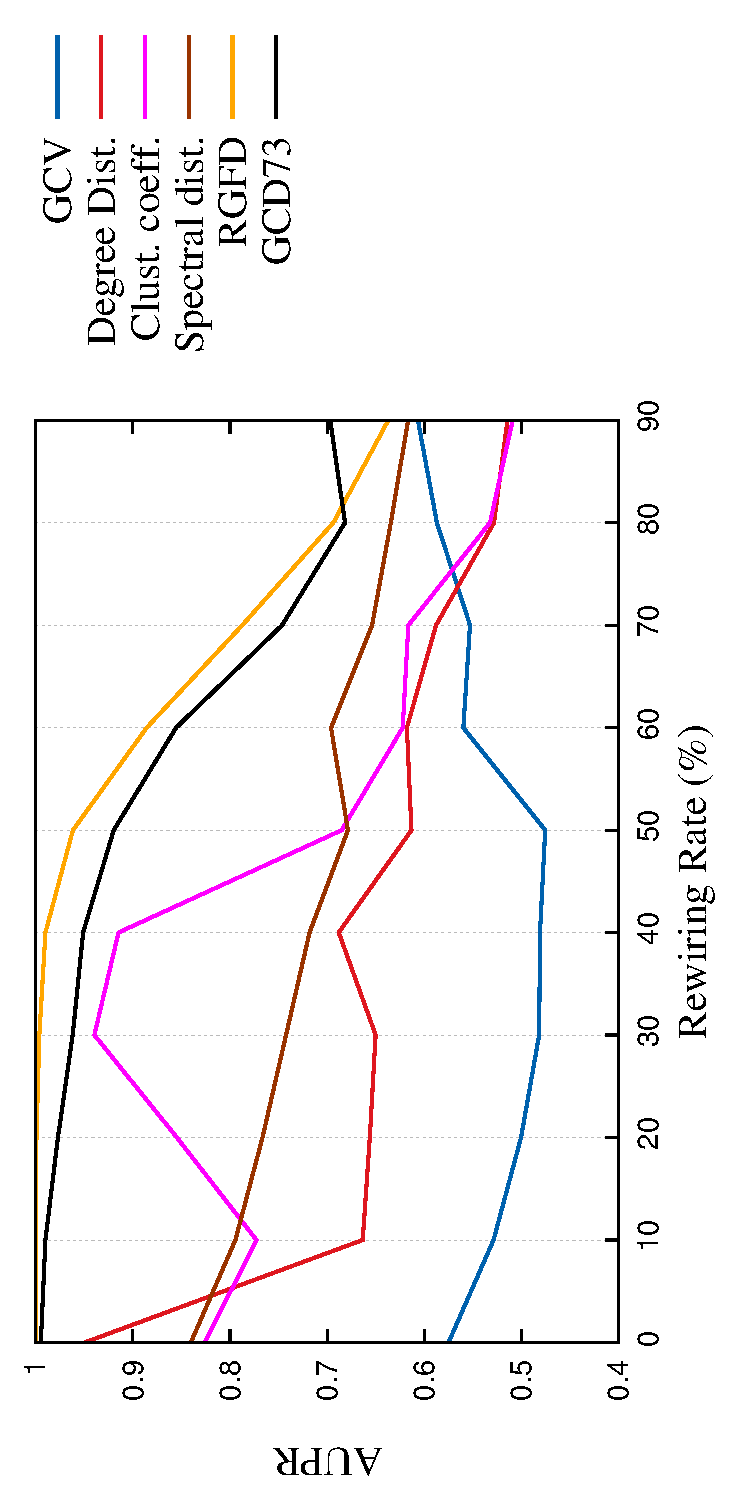
\includegraphics[scale=0.7, angle=-90]
  {../code/final_results/trade_2010_thresholded/eval_results/rew_aupr_all_sigs2.pdf}
  \caption[The AUPR for different percentages of noise in the model networks]{The AUPR for different percentages of noise in the model networks. The rewiring probability increases from 0 to 90\%. The GCV signature has a poor performance when dealing with noisy data, having the lowest AUPR when the rewiring parameter is in the [0--70] range.}
  \label{fig:rew_aupr}
\end{figure}

\subsection{Edge completeness}

In real-life situations, one also has to deal with incomplete data. In order to simulate incomplete data in our networks, we remove $q\%$ of the edges from the networks, where $q$ varies from 100\% (full network) to 10\% (incomplete network). Moreover, in order to simulate both noisy and incomplete data, we choose the 40\% rewired networks as the starting point and then start removing edges from these networks. We evaluate the performance of the signatures on these noisy and incomplete networks. 

\hilight{fix the p and q percentages fonts}

Figure \ref{fig:compl_aupr} shows the AUPR of the networks as the edge completeness parameter varies from 100\% to 10\%. The initial networks have been rewired with a 40\% probability. All the signatures display a general downward trend. The GCV signature performs poorly also in this experiment, always having an AUPR that is smaller than the AUPR of the other signatures. Some signatures such as the RGFD have a sharper drop in their AUPR than other signatures such as the Spectral Distribution. This suggests that RGFD is not as robust to incomplete data as the Spectral Distribution is. We conclude that the GCV signature is unable to deal with incomplete data either.

\begin{figure}[H]
  \hspace{-1.5em}
  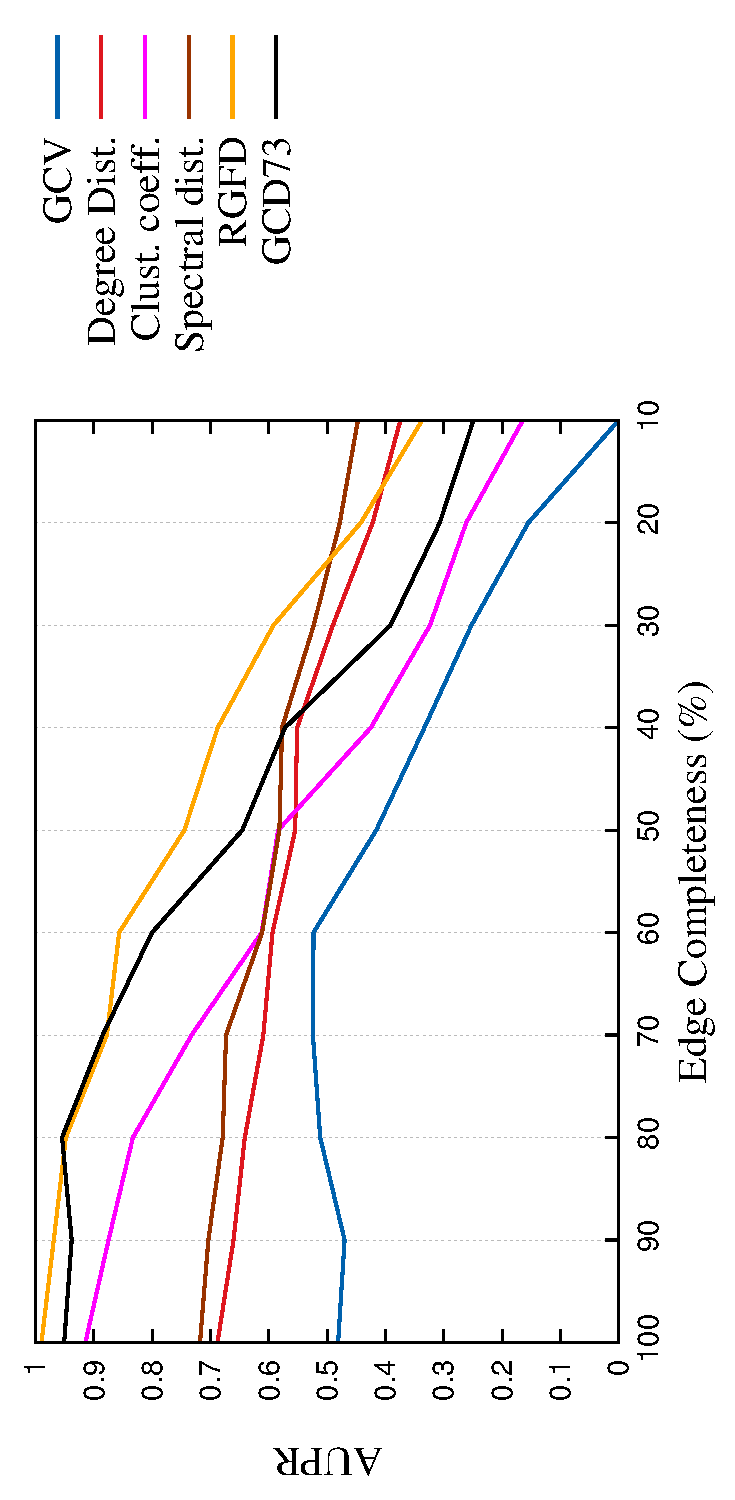
\includegraphics[scale=0.7, angle=-90]
  {../code/final_results/trade_2010_thresholded/eval_results/compl_aupr_all_sigs2.pdf}
  \caption[The AUPR for different percentages of edge completeness in the model networks]{The AUPR for different percentages of edge completeness in the model networks. The GCV signature also has a poor performance when dealing with incomplete data, always having the lowest AUPR compared to the other signatures.}
  \label{fig:compl_aupr}
\end{figure}

\subsection{Signature approximation}

In order to speed up computation, sometimes we have to approximate the signatures that are computed for all the random networks. In this section we try to evaluate the robustness of each signature to approximation. For each network, we only use a percentage $p\%$ of nodes to calculate the signatures. This is done for each signature/metric in the following manner:
\begin{enumerate}
 \item Graphlet Cluster Vector (GCV): We compute the Pearson's GCV correlation matrix using the GCV signatures of only $p\%$ of the nodes.
 \item Degree Distribution: We calculate the degree distribution from $p\%$ of the nodes in the graph.
 \item Average clustering coefficient: We average only the clustering coefficient of $p\%$ of the nodes.
 \item Spectral distribution: We compute the Laplacian matrix $L$ of the original network, then randomly sample $p\%$ nodes and take the submatrix $L'$ of $L$ that corresponds to the sampled nodes. We compute the spectral distribution from the submatrix $L'$.
 \item Graphlet Frequency Vector (used for computing RGFD): We randomly sample $p\%$ of the nodes and take the induced subgraph $S$ on these nodes. We then compute the GFV in $S$.
 \item GCD73: We compute the Graphlet correlation matrices using the GDV signatures of only $p\%$ of the nodes.  
\end{enumerate}

The experiments for signature approximation have also been run using the 40\% rewired networks, which simulate noisy data. The results are presented in figure \ref{fig:sampl_aupr}. For the GCV signature, we notice that it is actually robust to signature approximation, showing a very small but steady drop in the AUPR as less nodes are sampled. Other metrics such as the RGFD show a sharp drop in AUPR from 1.0 to 0.2, suggesting that RGFD is not robust to approximations. The Spectral distribution can also be considered robust, showing a peak AUPR of 0.7 when 50\% of the nodes are sampled. 

\begin{figure}[H]
  \hspace{-1.5em}
  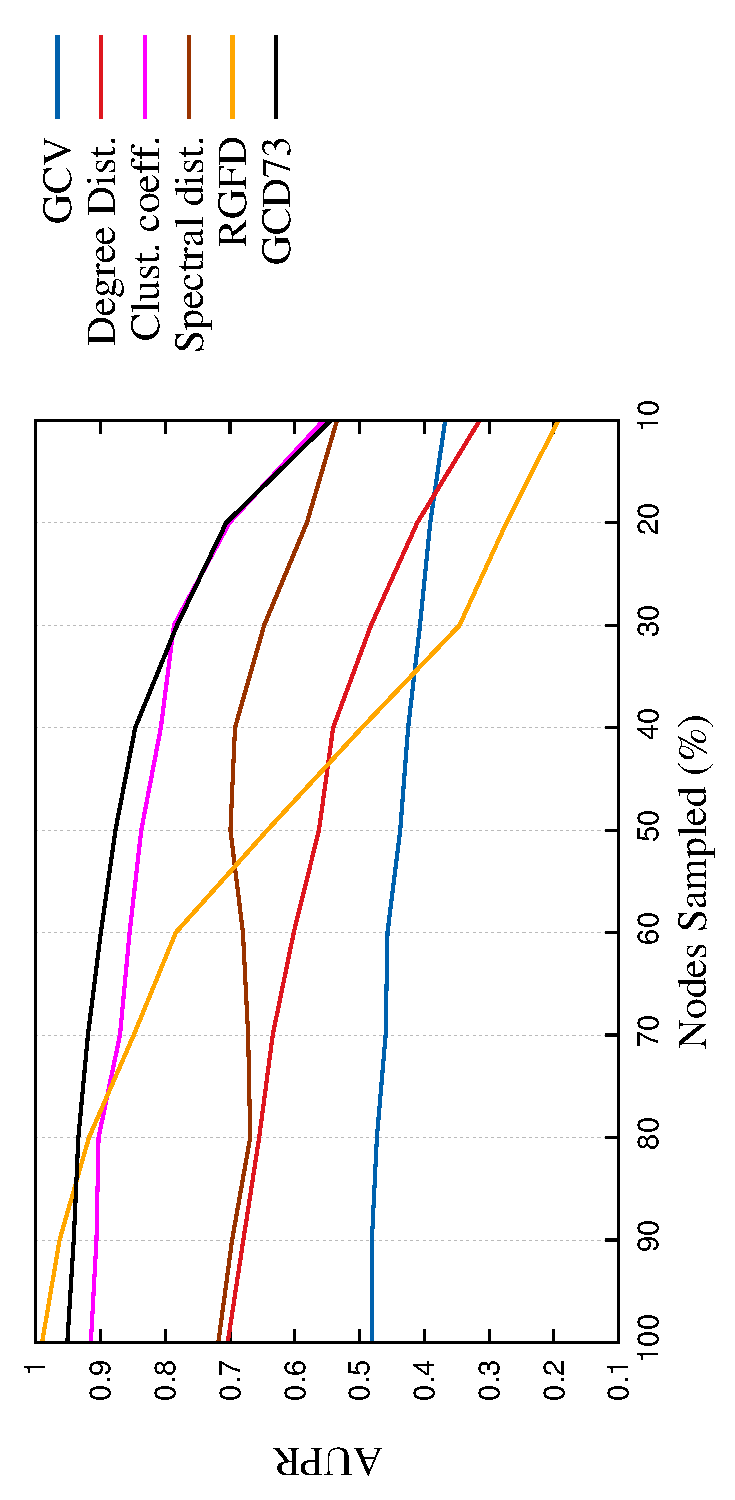
\includegraphics[scale=0.7, angle=-90]
  {../code/final_results/trade_2010_thresholded/eval_results/sampl_aupr_all_sigs2.pdf}
  \caption[The AUPR for different percentages of nodes sampled in the model networks]{The AUPR for different percentages of nodes sampled in the model networks. The GCV signature is robust to approximation, showing only a slight but steady drop in AUPR as the percentage of nodes sampled varies from 100\% to 10\%. On the other hand, the RGFD shows a sharp drop, suggesting that it is not robust to signature approximation.}
  \label{fig:sampl_aupr}
\end{figure}

In conclusion, the novel GCV signature is not robust to noisy or incomplete data, but it is robust to signature approximation. The signatures that performed best on our tests are the RGFD and GCD73, which are mostly robust to noisy and incomplete data.

\section{GCV-based Classifier}
\label{sec:eval_classify}

In this section we evaluate the performance of the GCV signature at classifying proteins into functional classes. We use Collin's Yeast AP-MS PPI network for computing the GCV of each protein.\footnote{The reason we run it on Collin's AP-MS network is because CCA analysis has given a high correlation on this dataset (see section \ref{sec:18_ppi_cca_results}).} Separately, we label each protein using Boone's annotation that comprises 14 different classes. The classifier we wrote uses a K-nearest neighbours (K-NN) method for predicting the function of a protein in the following manner:
\begin{itemize}
 \item Compute the GCV signature for all the proteins in the input network.
 \item For predicting the function of a given protein, compute the Euclidean distances between the GCV of the protein and the GCV of all the other proteins in the training data set. Store the distances in an array and sort it. 
 \item Find the closest $K$ data points to the input protein according to the computed distances.
 \item Perform majority voting\footnote{In majority voting, the class that has the highest frequency is the one that is returned. If two or more classes have the same highest frequency, one of them is chosen at random.} on the classes of the $K$ nearest neighbours and return the result as the predicted class.
\end{itemize}

This process is run inside a Cross-validation framework, where the protein dataset is split into two groups:
\begin{itemize}
 \item training data: this is stored in a data structure and is used for predicting the class of proteins using K-NN
 \item test data: this dataset is used for the actual prediction.
\end{itemize}

We split the dataset into 10 different chunks and run 10-fold cross-validation. We also choose $N = 5$ as the number of neighbours on which majority voting is performed. At each fold, 90\% of the data is used for training and 10\% for testing. For each fold during cross-validation, we compute a confusion matrix $M$ for all the classes, where entry $M(i,j)$ corresponds to the number of data points that have actual label $i$, but the classifier predicted them as having label $j$. The confusion matrices for each fold are added together and a final confusion matrix is obtained at the end of the cross-validation process. From the final confusion matrix, we then count for each class $C$ the following types of data points:
 \begin{itemize}
  \item \textbf{True Positives} ($TP$) are the data points that belong to $C$ and have also been correctly predicted as belonging to class $C$.
  \item \textbf{False Positives} ($FP$) the data points that do not belong to $C$ but have been incorrectly predicted as belonging to class $C$.
  \item \textbf{True Negatives} ($TN$) are the data points that not belong to $C$ and have also been correctly predicted as not belonging to class $C$.
  \item \textbf{False Negatives} ($FP$) the data points that do not belong to $C$ but have been incorrectly predicted as belonging to class $C$.
 \end{itemize}

After we compute the number of $TP$, $FP$, $TN$ and $FN$ data points, we can calculate for each class $C$ the following 3 statistics:
\begin{itemize}
 \item Precision: the percentage of data points that have been correctly classified in $C$ out of all the data points that have been classified in $C$. The exact formula for precision is:
 $$ Precision = \frac{TP}{TP + FP}$$
  \item Recall: the percentage of data points that have been correctly classified in $C$ out of all the data points are in $C$. It is formally defined as:
 $$ Recall = \frac{TP}{TP + FN}$$
  \item $F_1$ score: it is a measure of the test's accuracy that combines both precision and recall. The formula for $F_1$ is as follows:
 $$ F_1 = \frac{2 * Precision * Recall}{Precision + Recall}$$
 
\end{itemize}

\subsection{Classifier Results}

\definecolor{header}{HTML}{9DE6E6} % 
\definecolor{diag}{HTML}{05D1FF} % 

Figure \ref{fig:conf_matrix} shows the confusion matrix obtained for Collin's AP-MS Yeast PPI network using Boone's annotations. Note that only part of the classes have been tested in our classifier. The reason for this is because there were not enough data points for some classes to allow our algorithm to run properly. For example, there was only one sample belonging to the class \emph{Cell cycle progression/meiosis} in our dataset. As a result, we ran our classifier only on 9 classes that did not originally give an $F_1$ score of zero.\footnote{We first ran our classifier using all the classes and removed the classes for which the final $F_1$ score was zero.}

We observe that although our classifier correctly classified some data points (diagonal entries), there are considerable errors, especially in the first column (Nuclear transport). A considerable number of data entries have been incorrectly predicted as belonging to Nuclear transport, and we attribute this to the following bias in our methodology: during the majority voting phase, if two or more frequencies have the same highest score, the class with the lowest index is ultimately selected. As a result, the first class (Nuclear transport) is more likely to be selected as 
opposed to others. A closer look at the data further explains why some of the proteins are wrongly classified: there are many proteins that have the exact same GCV signature but different functional annotations. Most of these proteins tend to have a sparse neighbourhood, a fact that is easily noticed in the GCV signature, with many frequencies set to zero. 

On the other hand, we also notice that there is a large number of True Positives for RNA processing (RNA proc.), Chromatin transcription (Chrom. transc.) and Ribosome translation (Rib. transl.). Ribosome Translation and Chromatin transcription also had a large cross-loading magnitude in the CCA analysis (see figure \ref{yeast_apms_collins_cca}). We can therefore conclude that the GCV signature is particularly suitable for analysing proteins that are involved in Ribosome translation and Chromatin transcription.

Finally, the classifier has not correctly classified any protein labelled with DNA replication, as there are no True Positives for this class. The reason for this might be because we only use $N = 5$ nearest neighbours, and if the classifier finds at least 3 proteins from Nuclear Transport (Nucl. trans.) that have the same GCV signature as a protein that belongs to DNA replication, it will instead be assigned a Nuclear Transport label instead. We have tried using a value of $K$ that is bigger than 5, but that did not result in a better classification, having the final $F_1$ score approximately the same or lower.

\begin{figure}[H]
\centering
\begin{tabular}{p{2.7cm} p{1.0cm} p{1.0cm} p{1.0cm} p{1.0cm} p{1.0cm} p{1.0cm} p{1.0cm} p{1.0cm} p{1.0cm} }
\cellcolor{header} \backslashbox{actual}{pred.}  & \cellcolor{header} Nucl. trans.  & \cellcolor{header} Chrom. seg.  & \cellcolor{header} RNA proc.  & \cellcolor{header} Chrom. transc.  & \cellcolor{header} DNA repl.  & \cellcolor{header} Prot. deg.  & \cellcolor{header} Golgi sort.  & \cellcolor{header} Metab.  & \cellcolor{header} Rib. transl. \\

\cellcolor{header} Nucl. trans. &  \cellcolor{diag}  24 &  3 &  5 &  2 &  0 &  0 &  4 &  1 &  1\\ 

\cellcolor{header} Chrom. seg. &  41 &  \cellcolor{diag}  23 &  5 &  3 &  0 &  3 &  1 &  0 &  1\\ 

\cellcolor{header} RNA proc. &  42 &  11 &  \cellcolor{diag}  99 &  26 &  0 &  5 &  7 &  1 &  18\\ 

\cellcolor{header} Chrom. transc. &  62 &  21 &  20 &  \cellcolor{diag}  95 &  0 &  6 &  6 &  1 &  11\\ 

\cellcolor{header} DNA repl. &  67 &  10 &  1 &  3 &  \cellcolor{diag}  0 &  0 &  1 &  1 &  1\\ 

\cellcolor{header} Prot. deg. &  19 &  5 &  3 &  6 &  0 &  \cellcolor{diag}  18 &  0 &  0 &  0\\ 

\cellcolor{header} Golgi sort. &  63 &  21 &  2 &  13 &  0 &  0 &  \cellcolor{diag}  23 &  0 &  0\\ 

\cellcolor{header} Metab. &  72 &  4 &  4 &  2 &  0 &  0 &  2 &  \cellcolor{diag}  7 &  4\\ 

\cellcolor{header} Rib. transl. &  35 &  10 &  31 &  23 &  0 &  0 &  0 &  1 &  \cellcolor{diag}  60\\ 

\end{tabular}
\caption[Confusion matrix obtained on Collins AP-MS Yeast PPI network after 10-fold cross-validation.]{Confusion matrix obtained on Collins AP-MS Yeast PPI network after 10-fold cross-validation, using Boone's annotations as classes. The rows represent actual classes, while columns represent predicted classes. The classes used were: Nuclear transport (Nucl. trans.), Chromatin segmentation (Chrom. seg.), RNA processing (RNA proc.), Chromatin transcription (Chrom. transc.), DNA replication, repair, HR cohesion (DNA repl.), Protein degradation (Prot. deg.), Golgi endosome vacuole sorting (Golgi sort.), Metabolism - mitochondria (Metab.) and Ribosome translation (Rib. transl).}
\label{fig:conf_matrix}
\end{figure}

Table \ref{tab:prec_rec_f1_table} shows the Precision, Recall and $F_1$ rates for each of the 9 classes used by our classifier. At the bottom of the table, the average precision, recall and $F_1$ rates across all classes are shown. The results in the table show that the GCV-based classifier is not efficient at classifying proteins according to their function. The average precision and recall rates are only 0.41 and 0.31 respectively, while the average $F_1$ rate is 0.29. However, there is considerable variance in precision, recall and $F_1$ rates across the classes. For example, the classifier has a relatively high precision for classes such as Ribosome translation, Protein degradation, Golgi Endosome sorting and RNA processing. On the other hand, a class such as DNA replication has zero precision, meaning that no protein has been correctly classified to this class.

Overall, we conclude that the GCV-based K-NN classifier is not suitable for labelling proteins from PPI networks according to their function. Nevertheless, it still performs 3-4 times better than a random classifier, which would have average precision, recall and $F_1$ rates of around $\frac{1}{9} = 0.11$, when 9 classes are used. Last but not least, we also tried running the same classifier with different parameters $N$ -- nearest neighbours and $F$ -- fold numbers. When varying $N$, we got the best results when $N$ was in the range [5,10], although the performance decreases only slightly for $N$ greater than 10.

\begin{table}[H]
  \centering
  \begin{tabular}{  c | c  c  c }
    Class & Precision & Recall & F1\\
    \hline
    Nuclear-cytoplasmic transport & 0.056 & 0.600 & 0.103\\
    Chromatin segmentation  & 0.213 & 0.299 & 0.249\\
    RNA processing & 0.582 & 0.474 & 0.522\\
    Chromatin transcription & 0.549 & 0.428 & 0.481\\
    DNA replication, repair, HR cohesion & 0.000 & 0.000 & 0.000\\
    Protein degradation proteosome & 0.562 & 0.353 & 0.434\\
    Golgi endosome vacuole sorting & 0.523 & 0.189 & 0.277\\
    Metabolism - mitochondria & 0.583 & 0.074 & 0.131\\
    Ribosome translation & 0.625 & 0.375 & 0.469\\
    \hline
    Average & 0.410 & 0.310 & 0.296\\
  \end{tabular}
  \caption[Precision, recall and $F_1$ rates for each class used by the protein annotation classifier.]{Precision, recall and $F_1$ rates for each class used by the protein annotation classifier. At the bottom of the table, the overall average precision, recall and $F_1$ rates are given. The low scores in average precision (0.41), recall (0.31) and $F_1$ (0.29) suggest that our GCV-based classifier is not suitable for classifying proteins according to their function.}
  \label{tab:prec_rec_f1_table}
\end{table}

\section{Evaluation Summary}

We conclude that when clustering random networks generated with different algorithms, the GCV signature is not as efficient as other signatures or metrics. Nevertheless, the GCV can still be successfully used for data analysis and it helped us uncover interesting insights from the economic and biological networks. Moreover, the GCV might still be successfully used for clustering, if combined with other signatures such as the GDV.

Furthermore, our results do not precisely resemble those obtained by Yavero\u{g}lu et al. in 2014 \cite{yaverouglu2014revealing}. The reason for this is because we have not used the same source network to generate the random networks. Moreover, Yavero\u{g}lu et al. have also done the precision-recall curve analysis on a larger number of networks. In our case, we considered that 150 generated networks are sufficient to perform the analysis and draw our conclusions.

Section \ref{sec:eval_classify} also showed that the GCV signature cannot be directly used as a classifier without further modifications. The K-NN classifier we built for Collin's AP-MS Yeast PPI network using Boone's annotations is not precise and has a low $F_1$ score of 0.29. The reason for this is because there are several proteins that have the exact same GCV signature but different functional labels. We therefore suggest an improved GCV signature that captures more information about the protein's neighbourhood. One possibility is the combination of GDV and GCV signatures into one vector of frequencies. 
